%  !TeX  root  =  user_guide.tex

\chapter{Print Composer}\label{label_printcomposer}

% when the revision of a section has been finalized,
% comment out the following line:
% \updatedisclaimer

The print composer provides growing layout and printing
capabilities. It allows you to add elements such as the QGIS map canvas,
legend, scalebar, images, basic shapes, arrows and text labels. You can
size, group, align and position each element and adjust the properties to
create your layout. The layout can be printed or exported to image formats,
Postscript, PDF or to SVG \footnote{Export to SVG supported, but it is not working
properly with some recent QT4 versions. You should try and
check individual on your system} and you can save the layout as template and
load it again in another session. See a list of tools in
table~\ref{tab:printcomposer_tools}:

\begin{table}[h]\index{Print composer!tools}
\centering\small
\renewcommand{\arraystretch}{2}
 \begin{tabular}{|m{1cm}|m{5.4cm}|m{1cm}|m{5.4cm}|}
 \hline \textbf{Icon} & \textbf{Purpose} & \textbf{Icon} &
 \textbf{Purpose} \\
 \hline 
\includegraphics[width=0.7cm]{mActionFolder}
 & Load from template &
 
\includegraphics[width=0.7cm]{mActionFileSaveAs} & Save as template \\
 \hline 
\includegraphics[width=0.7cm]{mActionExportMapServer}
 & Export to an image format &
 
\includegraphics[width=0.7cm]{mActionSaveAsPDF} & Export as PDF \\
 \hline 
\includegraphics[width=0.7cm]{mActionSaveAsSVG} & Export print
 composition to SVG & 
\includegraphics[width=0.7cm]{mActionFilePrint}
 & Print or export as Postscript \\
 \hline 
\includegraphics[width=0.7cm]{mActionZoomFullExtent} & Zoom to
 full extend & 
\includegraphics[width=0.7cm]{mActionZoomIn} & Zoom in \\
 \hline 
\includegraphics[width=0.7cm]{mActionZoomOut} & Zoom out &
 
\includegraphics[width=0.7cm]{mActionDraw} & Refresh view \\
 \hline 
\includegraphics[width=0.7cm]{mActionAddMap} & Add new map from
 QGIS map canvas & 
\includegraphics[width=0.7cm]{mActionSaveMapAsImage}
 & Add Image to print composition \\
 \hline 
\includegraphics[width=0.7cm]{mActionLabel} & Add label to print
 composition & 
\includegraphics[width=0.7cm]{mActionAddLegend} & Add new
 legend to print composition \\
 \hline 
\includegraphics[width=0.7cm]{mActionScaleBar} & Add new scalebar
 to print composition & 
\includegraphics[width=0.7cm]{mActionAddBasicShape}
 & Add basic shape to print composition \\
 \hline 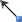
\includegraphics[width=0.7cm]{mActionAddArrow} & Add arrow to print
 composition & 
\includegraphics[width=0.7cm]{mActionOpenTable} & Add attribute
 table to print composition \\
 \hline 
\includegraphics[width=0.7cm]{mActionSelectPan} & Select/Move item in
 print composition &
 
\includegraphics[width=0.7cm]{mActionMoveItemContent} & Move content within
 an item \\
 \hline 
\includegraphics[width=0.7cm]{mActionGroupItems} & Group items of
 print composition &
 
\includegraphics[width=0.7cm]{mActionUngroupItems} & Ungroup items of print
 composition \\
 \hline 
\includegraphics[width=0.7cm]{mActionRaiseItems} & Raise selected
 items  &
 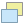
\includegraphics[width=0.7cm]{mActionLowerItems} & Lower selected items \\
 \hline 
\includegraphics[width=0.7cm]{mActionMoveItemsToTop} & Move selected
 items to top &
 
\includegraphics[width=0.7cm]{mActionMoveItemsToBottom} & Move selected
 items to bottom \\
 \hline 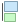
\includegraphics[width=0.7cm]{mActionAlignLeft} & Align selected
 items left &
 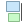
\includegraphics[width=0.7cm]{mActionAlignRight} & Align selected items
 right \\
 \hline 
\includegraphics[width=0.7cm]{mActionAlignHCenter} & Align selected
 items center &
 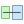
\includegraphics[width=0.7cm]{mActionAlignVCenter} & Align selected items
 center vertical \\
 \hline 
\includegraphics[width=0.7cm]{mActionAlignTop} & Align selected
 items top &
 
\includegraphics[width=0.7cm]{mActionAlignBottom} & Align selected
 items bottom \\
\hline
\end{tabular}
\caption{Print Composer Tools}\label{tab:printcomposer_tools}
\end{table}

All Print Composer tools are availabe in menus and as icons in a toolbar. The
toolbar can be switched off and on using the right mouse button holding the
mouse over the toolbar.

\section{Open a new Print Composer Template}\label{composertemplates}

Before you start to work with the print composer, you need to load some
raster and vector layers in the QGIS map canvas and adapt their properties
to suite your own convenience. After everything is rendered and symbolized to
your liking you click the \toolbtntwo{mActionNewComposer}{New Print Composer}
icon in the toolbar or choose \mainmenuopt{File} \arrow
\dropmenuopttwo{mActionNewComposer}{New Print Composer}.

\section{Using Print Composer}\label{label_useprintcomposer}

\begin{figure}[ht]
   \centering
   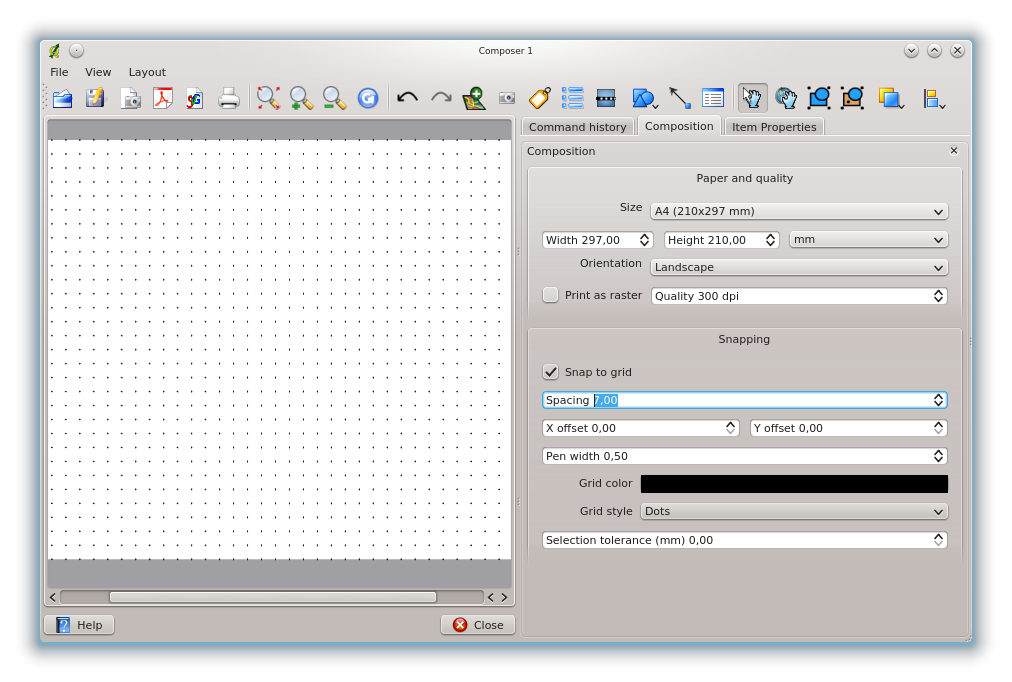
\includegraphics[clip=true, width=\textwidth]{print_composer_blank}
   \caption{Print Composer \nixcaption}\label{fig:print_composer_blank}
\end{figure}

Opening the print composer provides you with a blank canvas to which you can
add the current QGIS map canvas, legend, scalebar, images, basic shapes,
arrows and text. Figure \ref{fig:print_composer_blank} shows the initial view
of the print composer with an activated \checkbox{Snap to grid} modus but
before any elements are added. The print composer provides two tabs:

\begin{itemize}[label=--]
\item The \tab{General} tab allows you to set paper size, orientation, the
print quality for the output file in dpi and to activate snapping to a grid
of a defined resolution. Please note, the \checkbox{Snap to grid} feature
only works, if you define a grid resolution > 0. Furthermore you can also
activate the \checkbox{Print as raster} checkbox. This means all elements
will be rastered before printing or saving as Postscript of PDF.
\item The \tab{Item} tab displays the properties for the selected map element.
Click the \toolbtntwo{mActionSelectPan}{Select/Move item}
icon to select an element (e.g. legend, scalebar or label) on the canvas.
Then click the Item tab and customize the settings for the selected
element.
\end{itemize}

You can add multiple elements to the composer. It is also possible to have
more than one map view or legend or scalebar in the print composer canvas.
Each element has its own properties and in the case of the map, its own
extent.

\section{Adding a current QGIS map canvas to the Print Composer}

To add the QGIS map canvas, click on the \toolbtntwo{mActionAddMap}{Add new map
from QGIS map canvas} button in the print composer toolbar and drag a
rectangle on the composer canvas with the left mouse button to add the map.
To display the current map, you can choose between three different modes in
the map \tab{Item} tab:

\begin{itemize}[label=--]
\item \selectstring{Preview}{Rectangle} is the default setting. It only
displays an empty box with a message \textit{"Map will be printed here"}.
\item \selectstring{Preview}{Cache} renders the map in the current screen
resolution. If case you zoom in or out the composer window, the map is not
rendered again but the image will be scaled.
\item \selectstring{Preview}{Render} means, that if you zoom in or out the
composer window, the map will be rendered again, but for space reasons, only
up to a maximum resolution.
\end{itemize}

\textbf{Cache} is default preview mode for newly added print composer maps.

You can resize the map element by clicking on the
\toolbtntwo{mActionSelectPan}{Select/Move item} button, selecting the
element, and dragging one of the blue handles in the corner of the map. With
the map selected, you can now adapt more properties in the map \tab{Item}
tab.

To move layers within the map element select the map element, click
the \toolbtntwo{mActionMoveItemContent}{Move item content} icon
and move the layers within the map element frame with the left mouse button.
After you found the right place for an element, you can lock the element
position within the print composer canvas. Select the map element and click
on the right mouse button to \toolbtntwo{mIconLock}{lock} the element
position and again to unlock the element. You can lock the map element also
activating the \checkbox{Lock layers for map item} checkbox in the Map dialog
of the Map Item tab.

\textbf{Note:} QGIS \CURRENT is now able to show labels from the new labeling
plugin also in the map composer, but it is not yet scaled correctly. So it
might be necessary to switch back to the standard labeling in some cases.

\subsection{Map item tab - Map and Extents dialog}

\begin{figure}[ht]
  \centering
  \subfloat[Map dialog]{\label{subfig:map_dialog1}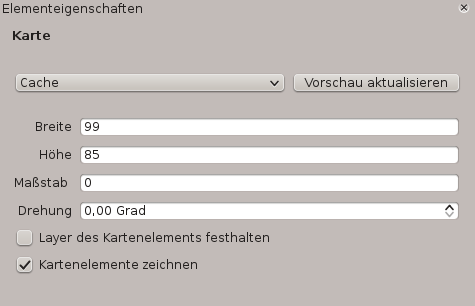
\includegraphics[clip=true, width=0.4\textwidth]{print_composer_map1}}
    \hspace{1cm}
  \subfloat[Extents dialog]{\label{subfig:map_dialog2}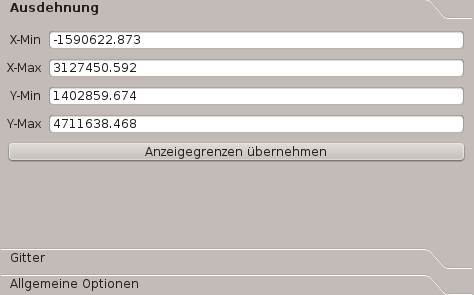
\includegraphics[clip=true, width=0.4\textwidth]{print_composer_map2}}
  \caption{Print Composer map item tab - Map and Extents dialog \nixcaption}\label{fig:mapdialog}
\end{figure}

\minisec{Map dialog}

The \textbf{Map} dialog of the map item tab provides following functionalities
(see Figure \ref{fig:mapdialog}a)):

\begin{itemize}[label=--]
\item The \textbf{Preview} area allows to define the preview modes Rectangle,
Cache and Render, as described above. Click on the \button{Update preview}
button to apply changes to the map view.
\item The \textbf{Map} area allows to resize the map element specifying the
width and height or the scale. The \selectstring{Rotation}{0} field allows to
rotate the map element content clockwise in degrees. Note, a coordinate frame
can only be added with the default value 0.
\end{itemize}

If you change the view on the QGIS map canvas by zooming or panning or
changing vector or raster properties, you can update the print composer view
selecting the map element in the print composer and clicking the
\button{Update preview} button.

\minisec{Extents dialog}

The \textbf{Extents} dialog of the map item tab provides following functionalities
(see Figure \ref{fig:mapdialog}b)):

\begin{itemize}[label=--]
\item The \textbf{Map extent} area allow to specify the map extent using Y
and X min/max values or clicking the \button{Set to map canvas extent} button.
\end{itemize}

If you change the view on the QGIS map canvas by zooming or panning or
changing vector or raster properties, you can update the print composer view
selecting the map element in the print composer and clicking the
\button{Update preview} button in the map \tab{Item} tab (see
Figure~\ref{fig:mapdialog}a)).

\subsection{Map item tab - Grid and General options dialog}

\begin{figure}[ht]
\centering
   \subfloat[Grid dialog]{\label{subfig:map_dialog3}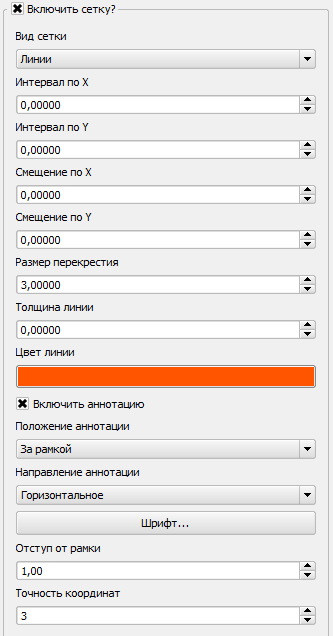
\includegraphics[clip=true, width=0.4\textwidth]{print_composer_map3}}
   \hspace{1cm}
   \subfloat[General options dialog]{\label{subfig:map_dialog4}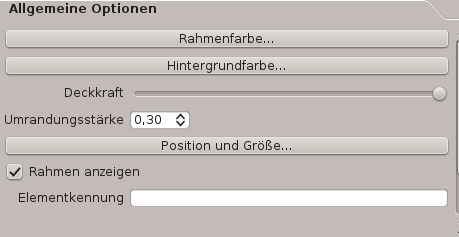
\includegraphics[clip=true, width=0.4\textwidth]{print_composer_map4}}
   \caption{Print Composer map item tab - Grid and General options dialog \nixcaption}\label{fig:sec_map_dialog}
\end{figure}

\minisec{Grid dialog}

The \textbf{Grid} dialog of the map item tab provides following functionalities
(see Figure \ref{fig:sec_map_dialog}a)):

\begin{itemize}[label=--]
\item The \checkbox{Show grid} checkbox allows to overlay a grid to the map
element. As grid type you can specify to use solid line or cross. Furthermore
you can define an interval in X and Y direction, an X and Y offset, and the
width used for cross or line grid type.
\item The \checkbox{Draw annotation} checkbox allows to add coordinates to
the map frame. The annotation can be drawn inside or outside the map frame.
As annotation direction can be defined horizontal, vertical, horizontal and
vertical or boundary direction. And finally you can define the grid color,
the annotation font, the annotation distance from the map frame and the
precision of the drawn coordinates.
\end{itemize}

\minisec{General options dialog}

The \textbf{General options} dialog of the map item tab provides following
functionalities (see Figure \ref{fig:sec_map_dialog}b)):

\begin{itemize}[label=--]
\item Here you can define color and outline width for the element frame, set
a background color and opacity for the map canvas. The \button{Position}
button opens the \dialog{Set items position} dialog and allows to set the map
canvas position using reference points or coordinates. Furthermore you can
select or unselect to display the element frame with the \checkbox{Show
frame} checkbox.
\end{itemize}

\section{Adding other elements to the Print Composer}

Besides adding a current QGIS map canvas to the Print Composer, it is also possible
to add, position, move and customize legend, scalebar, images and label elements.

\subsection{Label item tab - Label and General options dialog}

To add a label, click the \toolbtntwo{mActionLabel}{Add label} icon, place
the element with the left mouse button on the print composer canvas and
position and customize their appearance in the label item tab.

\begin{figure}[ht]
\centering
   \subfloat[label options dialog]{\label{subfig:labeloptions1}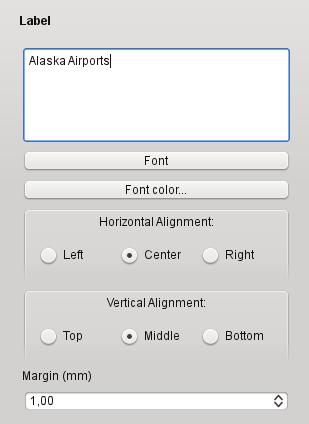
\includegraphics[clip=true, width=0.4\textwidth]{print_composer_label1}}
   \hspace{1cm}
   \subfloat[general options dialog]{\label{subfig:labeloptions2}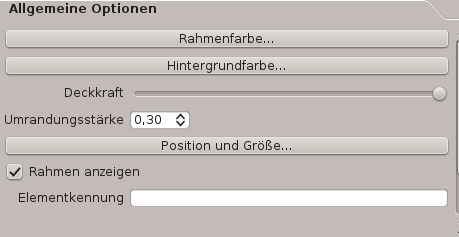
\includegraphics[clip=true, width=0.4\textwidth]{print_composer_label2}}
   \caption{Print composer label item tab - Label options and General options dialog \nixcaption}\label{fig:label_option}
\end{figure}

\minisec{Label dialog}

The \textbf{Label} dialog of the label item tab provides following
functionalities (see Figure \ref{fig:label_option}a)):

\begin{itemize}[label=--]
\item The \textbf{Label} dialog offers to add text labels to the composer
canvas. You can select font and fontcolor for the text and it is possible to
define a text margin im mm.
\end{itemize}

\minisec{General options dialog}

The \textbf{General options} dialog of the label item tab provides following
functionalities (see Figure \ref{fig:label_option}b)):

\begin{itemize}[label=--]
\item Here you can define color and outline width for the element frame, set
a background color and opacity for the label. The \button{Position}
button opens the \dialog{Set items position} dialog and allows to set the map
canvas position using reference points or coordinates. Furthermore you can
select or unselect to display the element frame with the \checkbox{Show
frame} checkbox.
\end{itemize}

\subsection{Image item tab - Picture options and General options dialog}

To add an image, click the \toolbtntwo{mActionSaveMapAsImage}{Add image}
icon, place the element with the left mouse button on the print composer
canvas and position and customize their appearance in the image item tab.

\begin{figure}[ht]
\centering
   \subfloat[Picture options dialog]{\label{subfig:print_composer_image1}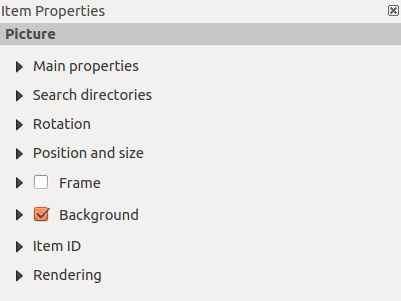
\includegraphics[clip=true, width=0.30\textwidth]{print_composer_image1}}
     \hspace{1cm}
   \subfloat[General options dialog]{\label{subfig:print_composer_image2}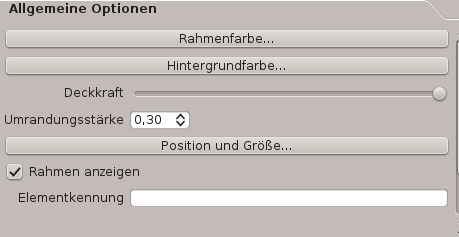
\includegraphics[clip=true, width=0.4\textwidth]{print_composer_image2}}
   \caption{Print composer image item tab - Picture options and General options \nixcaption}\label{fig:imageoptions}
\end{figure}

\minisec{Picture options dialog}

The \textbf{Picture options} dialog of the image item tab provides following
functionalities (see Figure \ref{fig:imageoptions}a)):

\begin{itemize}[label=--]
\item The \textbf{Search directories} area allows to add and remove
directories with images in SVG format to the picture database.
\item The \textbf{Preview} field then shows all pictures stored in the
selected directories.
\item The \textbf{Options} area shows the current selected picture and allows
to define width, height and clockwise rotation of the picture. It is also possible
to add a user specific SVG path. Activating the
\checkbox{Sync from map} checkbox synchronizes the rotation of a picture in
the qgis map canvas (i.e. a rotated north arrow) with the appropriate print
composer image.
\end{itemize}

\minisec{General options dialog}

The \textbf{General options} dialog of the image item tab provides following
functionalities (see Figure \ref{fig:imageoptions}b)):

\begin{itemize}[label=--]
\item Here you can define color and outline width for the element frame, set
a background color and opacity for the picture. The \button{Position}
button opens the \dialog{Set items position} dialog and allows to set the map
canvas position using reference points or coordinates. Furthermore you can
select or unselect to display the element frame with the \checkbox{Show
frame} checkbox.
\end{itemize}

\subsection{Legend item tab - General, Legend items and Item option dialog }

To add a map legend, click the \toolbtntwo{mActionAddLegend}{Add new legend}
icon, place the element with the left mouse button on the print composer
canvas and position and customize their appearance in the legend item tab.

\begin{figure}[h]
\centering
   \subfloat[General dialog]{\label{subfig:print_composer_legend1}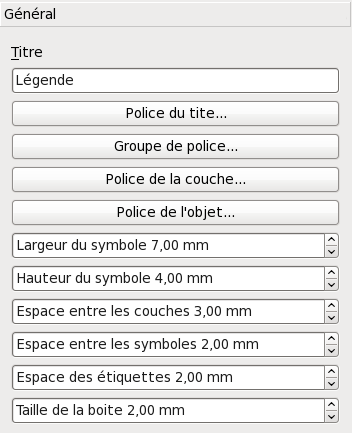
\includegraphics[clip=true, width=0.3\textwidth]{print_composer_legend1}}
   \hspace{1cm}
   \subfloat[Legend item dialog]{\label{subfig:print_composer_legend2}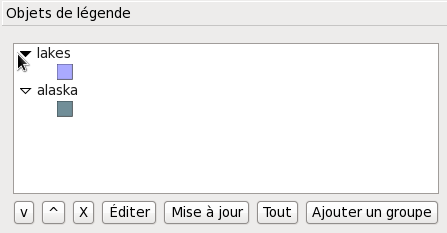
\includegraphics[clip=true, width=0.3\textwidth]{print_composer_legend2}}
   \hspace{1cm}
   \subfloat[Item options dialog]{\label{subfig:print_composer_legend3}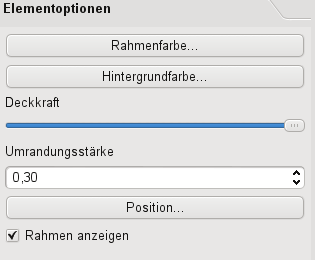
\includegraphics[clip=true, width=0.3\textwidth]{print_composer_legend3}}
   \caption{Print composer legend item tab - General, Legend items and Item option dialog\nixcaption}\label{fig:legendoptions}
\end{figure}

\minisec{General dialog}

The \textbf{General} dialog of the legend item tab provides following
functionalities (see Figure \ref{fig:legendoptions}a)):

\begin{itemize}[label=--]
\item Here you can adapt the legend title. You can change the font of the
legend title, layer and item name. You can change width and height of the
legend symbol and you can add layer, symbol, icon label and box space.
\end{itemize}

\minisec{Legend items dialog}

The \textbf{Legend items} dialog of the legend item tab provides following
functionalities (see Figure \ref{fig:legendoptions}b)):

\begin{itemize}[label=--]
\item The legend items window lists all legend items and allows to change
item order, edit layer names, remove and restore items of the list. After
changing the symbology in the QGIS main window you can click on \button{Update} to
adapt the changes in the legend element of the print composer. The item order
can be changed using the \button{Up} and \button{Down} buttons or with Drag and Drop
functionality.
\end{itemize}

\minisec{Item options dialog}

The \textbf{Item options} dialog of the legend item tab provides following
functionalities (see Figure \ref{fig:legendoptions}c)):

\begin{itemize}[label=--]
\item Here you can define color and outline width for the element frame, set
a background color and opacity for the legend. The \button{Position}
button opens the \dialog{Set items position} dialog and allows to set the map
canvas position using reference points or coordinates. Furthermore you can
select or unselect to display the element frame with the \checkbox{Show
frame} checkbox.
\end{itemize}

\subsection{Scalebar item tab - Scalebar and General options dialog}

To add a scalebar, click the \toolbtntwo{mActionScaleBar}{Add new scalebar}
icon, place the element with the left mouse button on the print composer
canvas and position and customize their appearance in the scalebar item tab.

\begin{figure}[ht]
\centering
\subfloat[scalebar options dialog]{\label{subfig:scalebaroptions1}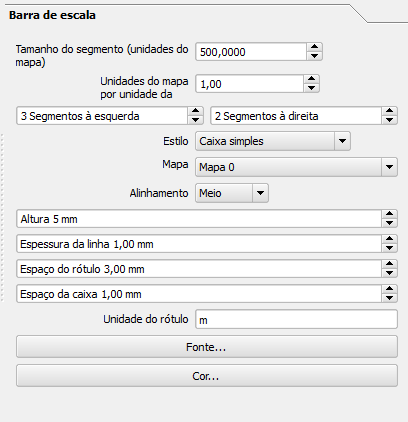
\includegraphics[clip=true, width=0.35\textwidth]{print_composer_scalebar1}}
\hspace{1cm}
\subfloat[general options dialog]{\label{subfig:scalebaroptions2}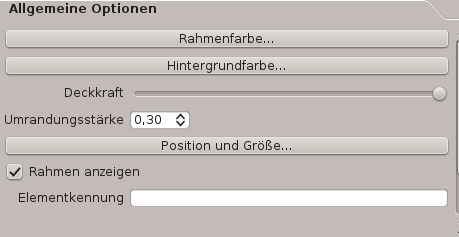
\includegraphics[clip=true, width=0.4\textwidth]{print_composer_scalebar2}}
\caption{Print composer scalebar item tab - Scalebar and General options dialog \nixcaption}\label{fig:scalebaroptions}
\end{figure}

\minisec{Scalebar dialog}

The \textbf{Scalebar} dialog of the scalebar item tab provides following
functionalities (see Figure \ref{fig:scalebaroptions}a)):

\begin{itemize}[label=--]
\item The scalebar dialog allows to define the segment size of the scalebar
in map units, the map units used per bar units, and how many left and right
segments units from 0 should be used.
\item You can define the scalebar style, available is single and double box,
line ticks middle, up and down and a numeric style.
\item Furthermore you can define height, line width, label and box space of
the scale bar. Add a unit label and define the scalebar font and color.
\end{itemize}

\minisec{General options dialog}

The \textbf{General options} dialog of the scalebar item tab provides following
features (see Figure \ref{fig:scalebaroptions}b)):

\begin{itemize}[label=--]
\item Here you can define color and outline width for the element frame, set
a background color and opacity for the scalebar. The \button{Position}
button opens the \dialog{Set items position} dialog and allows to set the map
canvas position using reference points or coordinates. Furthermore you can
select or unselect to display the element frame with the \checkbox{Show
frame} checkbox.
\end{itemize}

\section{Navigation tools}

For map navigation the print composer provides 4 general tools:

\begin{itemize}[label=--]
\item \toolbtntwo{mActionZoomIn}{Zoom in},
\item \toolbtntwo{mActionZoomOut}{Zoom out},
\item \toolbtntwo{mActionZoomFullExtent}{Zoom to full extend} and
\item \toolbtntwo{mActionDraw}{Refresh the view}, if you find the view in an
inconsistent state.
\end{itemize}

\section{Add Basic shape and Arrow}

It is possible to add basic shapes (Ellipse, Rectangle, Triangle) and arrows
to the print composer canvas.

\begin{figure}[ht]
\centering
\subfloat[shape dialog]{\label{subfig:shapedialog}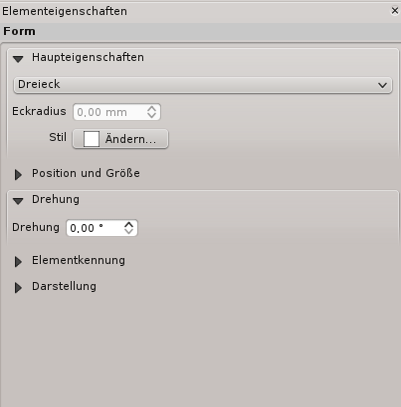
\includegraphics[clip=true, width=0.4\textwidth]{print_composer_shape}}
\hspace{1cm}
\subfloat[arrow dialog]{\label{subfig:arrowdialog}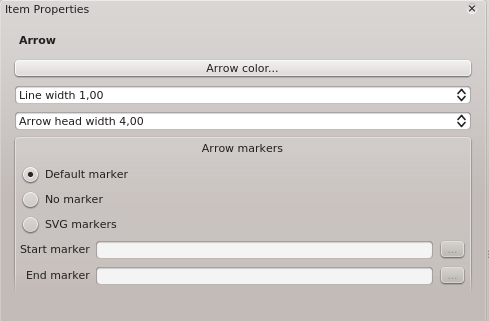
\includegraphics[clip=true, width=0.4\textwidth]{print_composer_arrow}}
\caption{Print composer basic shape and arrow item tab - Shape and Arrow options dialog \nixcaption}\label{fig:shapearrow}
\end{figure}

\begin{itemize}[label=--]
\item The \textbf{Shape} dialog allows to draw an ellipse, rectangle, or
triangle in the print composer canvas. You can define its outline and fill
color, the outline width and a clockwise rotation.
\item The \textbf{Arrow} dialog allows to draw an arrow in the print composer
canvas. You can define color, outline and arrow width and it is possible to
use a default marker and no marker and a SVG marker. For the SVG marker you
can additionally add a SVG start and end marker from a directory on your
computer.
\end{itemize}

\section{Add attribute table values}

It is possible to add parts of a vector attribute table to the print composer canvas.

\begin{figure}[ht]
\centering
\subfloat[table dialog]{\label{subfig:tabledialog1}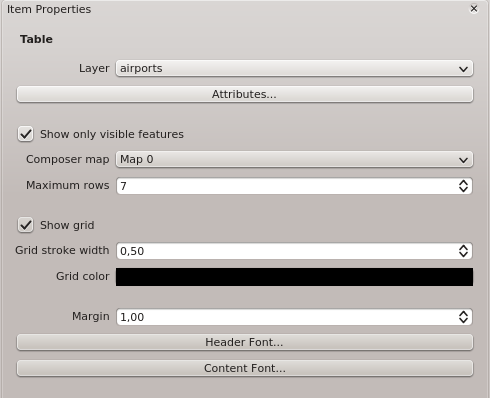
\includegraphics[clip=true, width=0.38\textwidth]{print_composer_attribute1}}
\hspace{1cm}
\subfloat[general options dialog]{\label{subfig:tabledialog2}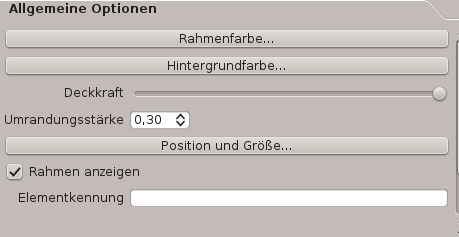
\includegraphics[clip=true, width=0.38\textwidth]{print_composer_attribute2}}
\caption{Print composer attribute table item tab - Table and General options dialog \nixcaption}\label{fig:attrcomp}
\end{figure}

\minisec{Table dialog}

The \textbf{Table} dialog of the attribute table item tab provides following
functionalities (see Figure \ref{fig:attrcomp}a)):

\begin{itemize}[label=--]
\item The \textbf{Table} dialog allows to select the vector layer and columns of
the attribute table. You can define the maximum number of rows to be displayed
and if attributes are only shown for visible features of the current composer
canvas. Additionally you can define the grid characteristics of the table and
the header and content font.
\end{itemize}

\minisec{General options dialog}

The \textbf{General options} dialog of the attribute table item tab
provides following functionalities (see Figure \ref{fig:attrcomp}b)):

\begin{itemize}[label=--]
\item Here you can define color and outline width for the element frame, set
a background color and opacity for the table. The \button{Position}
button opens the \dialog{Set items position} dialog and allows to set the map
canvas position using reference points or coordinates. Furthermore you can
select or unselect to display the element frame with the \checkbox{Show
frame} checkbox.
\end{itemize}

\section{Raise, lower and align elements}

Raise or lower functionalities for elements are inside the
\toolbtntwo{mActionRaiseItems}{Raise selected items} pulldown menu. Choose an
element on the print composer canvas and select the matching functionality to
raise or lower the selected element compared to the other elements (see
table~\ref{tab:printcomposer_tools}).

There are several alignment functionalities available within the
\toolbtntwo{mActionAlignLeft}{Align selected items} pulldown menu (see
table~\ref{tab:printcomposer_tools}). To use an alignment functionality , you
first select some elements and then click on the matching alignment icon. All
selected will then be aligned within to their common bounding box.

\section{Creating Output}

Figure \ref{fig:print_composer_complete} shows the print composer with an example
print layout including each type of map element described in the sections above.

\begin{figure}[h]
   \centering
   \includegraphics[clip=true, width=\textwidth]{print_composer_complete}
   \caption{Print Composer with map view, legend, scalebar, coordinates and text added \nixcaption} \label{fig:print_composer_complete}
\end{figure}

The print composer allows you to create several output formats and it is possible to
define the resolution (print quality) and paper size:

\begin{itemize}[label=--]
\item The \toolbtntwo{mActionFilePrint}{Print} icon allows to print the layout
to a connected printer or a Postscript file depending on installed printer
drivers.
\item The \toolbtntwo{mActionExportMapServer}{Export as image} icon exports the
composer canvas in several image formats such as PNG, BPM, TIF, JPG, \dots
\item The \toolbtntwo{mActionSaveAsPDF}{Export as PDF} saves the defined
print composer canvas directly as a PDF.
\item The \toolbtntwo{mActionSaveAsSVG}{Export as SVG} icon saves the print
composer canvas as a SVG (Scalable Vector Graphic). \textbf{Note:} Currently the
SVG output is very basic. This is not a QGIS problem, but a problem of the underlaying
Qt library. This will hopefully be sorted out in future versions.
\end{itemize}

\section{Saving and loading a print composer layout}

With the \toolbtntwo{mActionFileSaveAs}{Save as template} and
\toolbtntwo{mActionFolder}{Load from template} icons you can save the current
state of a print composer session as a  *.qpt template and load the template
again in another session.

The  \toolbtntwo{mActionComposerManager}{Composer Manager} button in the
toolbar and in \mainmenuopt{File} \arrow
\dropmenuopttwo{mActionComposerManager}{Composer Manager} allows to manage
add new composer template or to manage already existing templates.

\begin{figure}[h]
   \centering
   \includegraphics[clip=true, width=8cm]{print_composer_manager}
   \caption{Composer Manager \nixcaption}
   \label{fig:print_composer_manager}
\end{figure}

\FloatBarrier
